

\section{Comparison of 3D rendering technologies}
\setauthor{Romeo Bhuiyan}
In order to display a virtual model on a canvas, a 3D rendering technology was required. Two libraries, 
GLTFLoader and WebGL, were evaluated using JavaScript to determine the best fit for the task at hand. 
The choice between the two ultimately depends on the specific needs and limitations of the project. 
Both GLTFLoader and WebGL are effective tools for rendering, but each have their own 
unique strengths and weaknesses.
\\
\\
\subsection{WebGL}
\setauthor{Romeo Bhuiyan}
\textbf{WebGL} is designed to work seamlessly with other web technologies such as HTML, CSS, and JavaScript, 
making it easy to integrate 3D graphics into web pages. It allows developers to create a wide range 
of interactive 3D applications and visualizations, including games, scientific 
simulations, data visualizations, and more.
One of the key features of WebGL is its ability to take full advantage of the GPU 
(graphics processing unit) on the user's device. This allows WebGL applications to 
run smoothly and efficiently, even on devices with limited resources. Additionally, WebGL provides 
a high level of compatibility across different browsers and devices, making it a widely accessible technology.
WebGL is supported by most modern web browsers, including Chrome, Firefox, Safari, and Edge. 
This means that developers can create WebGL applications that can be easily accessed by 
users on a wide range of devices and platforms.
\\
\\
\subsection{GLTFLoader}
\setauthor{Romeo Bhuiyan}
\textbf{GLTFLoader} is a JavaScript library that allows developers to load and parse 3D models in the GLTF 
(GL Transmission Format) file format. GLTF is a widely adopted file format for 3D models and is 
supported by many 3D modeling software, including Blender and SketchUp.
GLTFLoader provides a simple and easy-to-use API for loading and parsing GLTF models, 
which can then be displayed using WebGL. The library takes care of all the complex tasks 
involved in loading and parsing the model data, such as handling binary buffers, parsing 
JSON data and creating the geometry and materials for the model.
GLTFLoader also provides support for advanced features such as animations, skinning and morph 
targets, which are typically found in more complex 3D models. This allows developers to create 
more advanced and interactive 3D applications and visualizations.
One of the key benefits of using GLTFLoader is that it greatly simplifies the process of loading and 
displaying 3D models on the web. By using a standardized file format and a dedicated library, 
developers can focus on creating the logic and functionality of their application, rather than 
spending time on complex parsing and loading tasks.
Additionally, GLTF is a highly efficient format, which means that it can be loaded faster, 
and also the files are smaller in size, making it a great choice for loading 3D models on the web.
\\
\\
\subsection{Conclusion}
n conclusion, GLTFLoader is a powerful tool for creating 3D graphics for the web that 
offers several advantages over WebGL. One of the main benefits of using GLTFLoader is 
its ability to handle the loading and parsing of GLTF (GL Transmission Format) files, 
which are a widely-used format for 3D models. This eliminates the need for developers 
to write their own code to handle file loading and parsing, saving time and effort. 
Additionally, GLTFLoader provides a more streamlined and convenient way to work with 
3D models, as it allows developers to easily import and use pre-existing models rather 
than having to create them from scratch. Furthermore, GLTFLoader also supports various 
features such as animations, cameras, lights and many more which can be easily integrated 
with web pages. Therefore, it is more efficient and convenient for the purpose of Animotion 
to work with 3D models on the web, GLTFLoader is the best choice as seen below in the figure. \ref{fig:gltfloader}
\\
\\
\begin{figure}[htb]
    \centering
    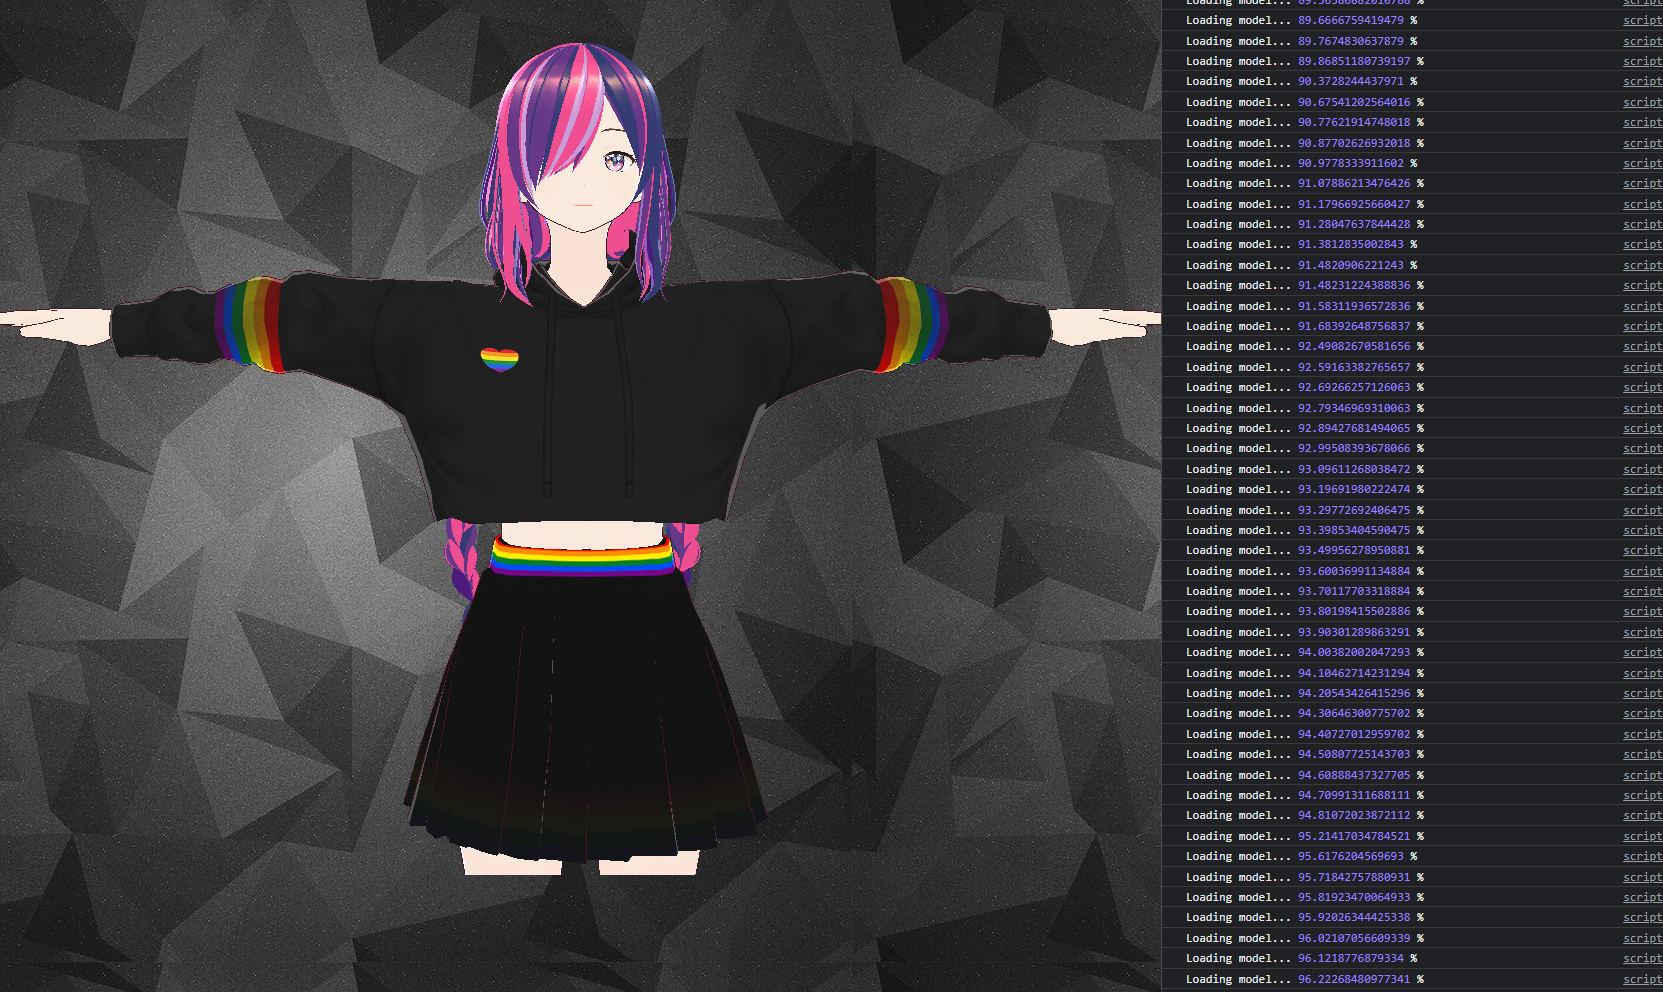
\includegraphics[width=0.9\textwidth]{pics/GLTFLoader.png}
    \caption{Loading the model with the help of GLTFLoader}
    \label{fig:gltfloader}
\end{figure}
\\
\\
\section{Calculation of the virtual reality model} 
\setauthor{Romeo Bhuiyan}
Controlling a VRM on a website involves a complex process that involves 
capturing the user's inputs, updating the VRMs position and orientation in real-time, 
and rendering the updated model for display on the user's device.
The first step in this process is for the user to interact with the VR model 
using a device such as a VR headset or a mouse and keyboard. The inputs from the 
user are then captured by the website and sent to the server. The server then 
uses these inputs to update the VR model's position and orientation in real-time. 
\\
\\
Once the VR model has been updated, it is then rendered, and the new frame is 
sent back to the user's device for display. This process repeats as the user 
continues to interact with the VR model. 
To achieve this, various technologies are needed such as GLTFLoader\cite{GLTFLoader} from the THREE\cite{threejs}
libraries for rendering the VR model in the browser, WebSockets for real-time 
communication between the client and server, and a physics engine to simulate 
the movement and interactions of the VR model. 
\\
\\
\subsection{Blendshape}
\setauthor{Romeo Bhuiyan}
Blendshape is a technique used in 3D animation and computer graphics to create a smooth transition between different shapes or expressions of a 3D model. 
It works by creating a set of "target" shapes for a 3D model, each representing a different expression or shape, 
and then using a set of weights or "blend" values to interpolate between these target shapes, creating a 
smooth transition between them. This allows animators to create a wide range of expressive characters with a 
limited number of 3D models. Blendshapes are commonly used in animation, film and game industry.
\\
\\
\subsection{Lerp}
\setauthor{Romeo Bhuiyan}
The Lerp function, short for Linear Interpolation, is a mathematical function that is 
used to smoothly blend between two values. The function takes three arguments: a start value, 
an end value, and a weight. The weight is a value between 0 and 1 that represents the proportion 
of the blend between the start and end values.
For example, if the weight is set to 0, the function will return the start 
value, and if the weight is set to 1, the function will return the end value. 
If the weight is set to 0.5, the function will return the midpoint between the 
start and end values. By adjusting the weight, the Lerp function can be used to 
smoothly transition between any two values over time.
In the context of computer graphics, Lerp function is widely used for 
interpolating values such as position, rotation, and color, to make the 
animation smooth. It's also used in physics simulations, game development, 
and other fields where the smooth transition of values is needed.
\\
\\
\subsection{Determining facial expressions using Blendshape techniques}
\setauthor{Romeo Bhuiyan}

\begin{lstlisting}[language=Python,caption=Shape of mouth,label=lst:shapeOfMouth]
    for each shape in ["I", "A", "E", "O", "U"]
        Blendshape.setValue(PresetName[shape], 
        lerp(riggedFace.mouth.shape[shape], 
        Blendshape.getValue(PresetName[shape]), 0.5))

\end{lstlisting}
This pseudocode \ref{lst:shapeOfMouth} is a loop that iterates over an array containing the shapes "I", "A", "E", "O", "U". 
The purpose of the loop is to blend the shape of a rigged face's mouth with a preset value of a 
Blendshape object for each of these shapes. The loop starts by setting the value of the Blendshape 
object to a blended value between the shape of the rigged face's mouth (riggedFace.mouth.shape[shape]) 
and the current value of the Blendshape object (Blendshape.getValue(PresetName[shape])). 
The blend is done using the lerp function, which stands for linear interpolation. 
This function takes three arguments: the start value, the end value, and the weight of blending. 
In this case, the weight is set to 0.5, resulting in an even blend between the two values.
Once the blended value is calculated, it is set to the Blendshape object using the PresetName 
as the key. This process is repeated for each shape in the array, allowing the developer to 
easily blend the shape of the rigged face's mouth with preset values for multiple shapes.
\\
\\
\begin{lstlisting}[language=Python,caption=Blinking of the eyes,label=lst:blinking]
    riggedFace.eye.l = lerp(clamp(1 - riggedFace.eye.l, 0, 1), Blendshape.getValue(PresetName.Blink), 0.5)
    riggedFace.eye.r = lerp(clamp(1 - riggedFace.eye.r, 0, 1), Blendshape.getValue(PresetName.Blink), 0.5)
    riggedFace.eye = Kalidokit.Face.stabilizeBlink(riggedFace.eye, riggedFace.head.y)
    Blendshape.setValue(PresetName.Blink, riggedFace.eye.l)

\end{lstlisting}
%insert text

%\begin{lstlisting}[language=Python,caption=Position of the model,label=lst:position]
%    function rigPosition(name, position={x:0, y:0, z:0}, dampener=1, lerpAmount=0.3) {
%        if (currentVrm is not defined) {
%          return;
%        }
%        Part = currentVrm.humanoid.getBoneNode(name from THREE.VRMSchema.HumanoidBoneName);
%        if (Part is not defined) {
%          return;
%        }
%        vector = new THREE.Vector3(position.x * dampener, position.y * dampener, position.z * dampener);
%        Part.position.lerp(vector, lerpAmount);
%    }
%      
%      oldLookTarget = new THREE.Euler();
%      function rigFace(riggedFace) {
%        if (currentVrm is not defined) {
%          return;
%        }
%        rigRotation("Neck", riggedFace.head, 0.7);
%      
%        Blendshape = currentVrm.blendShapeProxy;
%        PresetName = THREE.VRMSchema.BlendShapePresetName;
%    }
%      
%
%\end{lstlisting}
%text

